\documentclass[11pt]{article}
\usepackage[a4paper,margin=1in]{geometry}
\usepackage{graphicx}
\usepackage{booktabs}
\usepackage{tabularx}
\usepackage{hyperref}
\usepackage{amsmath}
\usepackage{tikz}
\usetikzlibrary{shapes.geometric, arrows.meta, positioning, calc, fit, backgrounds, decorations.pathreplacing}
\usepackage{xcolor}
\usepackage{float}

% Color palette
\definecolor{ceRed}{HTML}{E74C3C}
\definecolor{ieOrange}{HTML}{F39C12}
\definecolor{rcGreen}{HTML}{27AE60}
\definecolor{fcYellow}{HTML}{F1C40F}
\definecolor{naGray}{HTML}{95A5A6}
\definecolor{phase1Blue}{HTML}{3498DB}
\definecolor{phase2Green}{HTML}{2ECC71}
\definecolor{wbPurple}{HTML}{9B59B6}
\definecolor{lightbg}{HTML}{F8F9FA}

\title{White-Box Pipeline Report:\\
Detecting Self-Consistent Errors via Cross-Model Probing}
\author{Simranjeet Singh}
\date{March 9, 2026}

\begin{document}
\maketitle

% ============================================================
\section{Overview}
% ============================================================

This report summarizes what I built in the white-box portion of my pipeline and the method I adapted it from. The white-box pipeline is designed to detect \textbf{self-consistent errors} (CEs) in Large Language Models---cases where a model repeatedly gives the \emph{same wrong answer} with high confidence. These errors are particularly dangerous because the model shows no uncertainty, so traditional consistency-based detectors cannot catch them.

My implementation is based on the cross-model probing method introduced by Tan et al.\ in \emph{Too Consistent to Detect: A Study of Self-Consistent Errors in LLMs} (arXiv:2505.17656). I adapted their approach to work with my own evaluation setup on TruthfulQA across six LLM APIs.

% ============================================================
\section{What Tan et al.\ Did (The Original Method)}
% ============================================================

Tan et al.\ formally defined the concept of a \textbf{self-consistent error}: given a question, if the model's greedy answer is incorrect \emph{and} all stochastic samples (generated at temperature $T > 0$) are semantically equivalent to that greedy answer, then the response is a self-consistent error. The model is confidently wrong every time it is asked.

Their paper made two key empirical observations:
\begin{enumerate}
    \item \textbf{CEs do not decrease with model scale.} Unlike inconsistent errors, which tend to diminish as models get larger, CEs remain stable or even increase in frequency.
    \item \textbf{Existing detection methods struggle on CEs.} They evaluated four categories of detectors---consistency-based (e.g., semantic entropy), uncertainty-based, internal-state (white-box) probes, and hybrid approaches---and found substantial performance drops on CEs. Consistency-based detectors degraded the most, sometimes falling below random guessing (AUROC $\leq$ 0.5), because CEs produce low entropy by definition.
\end{enumerate}

To address this, Tan et al.\ proposed a \textbf{cross-model probe}. The core insight is that different models make different mistakes. They use a second ``verifier'' model alongside the original ``response'' model: both process the same question--answer pair, and a small probe is trained on each model's hidden states. The two probe scores are fused:
\[
    s_{\text{fused}} = (1 - \lambda) \cdot s_M + \lambda \cdot s_V
\]
where $s_M$ is the response model's probe score, $s_V$ is the verifier's, and $\lambda$ is tuned on a validation set. They showed this fused probe outperforms single-model probes, especially on CEs.

% ============================================================
\section{What I Did (My White-Box Pipeline)}
% ============================================================

I adapted the cross-model probe method from Tan et al.\ and built it into my existing two-phase evaluation pipeline. The overall architecture is shown in Figure~\ref{fig:pipeline}.

% --- Pipeline Architecture Diagram ---
\begin{figure}[H]
\centering
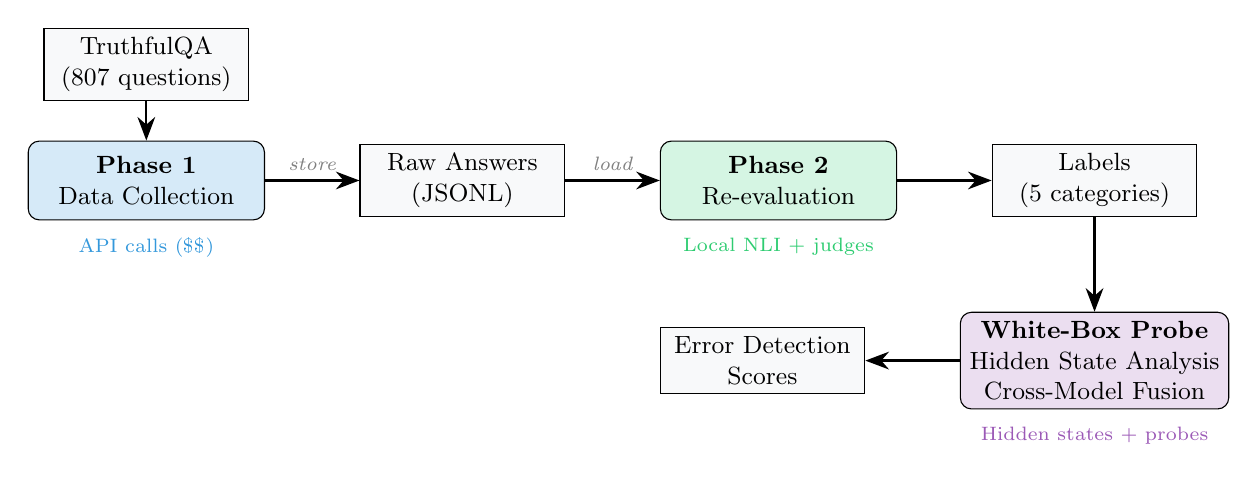
\begin{tikzpicture}[
    node distance=0.6cm and 1.2cm,
    box/.style={rectangle, draw, rounded corners=4pt, minimum width=3cm, minimum height=1cm, align=center, font=\small},
    data/.style={rectangle, draw, fill=lightbg, minimum width=2.6cm, minimum height=0.7cm, align=center, font=\small},
    arrow/.style={-{Stealth[length=3mm]}, thick},
    label/.style={font=\scriptsize\itshape, text=gray}
]
    % Phase 1
    \node[box, fill=phase1Blue!20] (p1) {\textbf{Phase 1}\\Data Collection};
    \node[data, right=of p1] (jsonl) {Raw Answers\\(JSONL)};
    \node[box, fill=phase2Green!20, right=of jsonl] (p2) {\textbf{Phase 2}\\Re-evaluation};
    \node[data, right=of p2] (labels) {Labels\\(5 categories)};

    % White-box
    \node[box, fill=wbPurple!20, below=1.2cm of labels] (wb) {\textbf{White-Box Probe}\\Hidden State Analysis\\Cross-Model Fusion};
    \node[data, left=of wb] (scores) {Error Detection\\Scores};

    % Input
    \node[data, above=0.5cm of p1] (tqa) {TruthfulQA\\(807 questions)};

    % Arrows
    \draw[arrow] (tqa) -- (p1);
    \draw[arrow] (p1) -- node[above, label] {store} (jsonl);
    \draw[arrow] (jsonl) -- node[above, label] {load} (p2);
    \draw[arrow] (p2) -- (labels);
    \draw[arrow] (labels) -- (wb);
    \draw[arrow] (wb) -- (scores);

    % Phase labels
    \node[below=0.1cm of p1, font=\scriptsize, text=phase1Blue] {API calls (\$\$)};
    \node[below=0.1cm of p2, font=\scriptsize, text=phase2Green] {Local NLI + judges};
    \node[below=0.1cm of wb, font=\scriptsize, text=wbPurple] {Hidden states + probes};
\end{tikzpicture}
\caption{Two-phase pipeline architecture with white-box probe. Phase~1 generates answers (expensive API calls). Phase~2 labels them using local NLI and judge ensembles. The white-box probe then uses hidden states to detect errors.}
\label{fig:pipeline}
\end{figure}

% --- 2x2 Error Matrix ---
\subsection{The Error Classification}

Every LLM response falls into one of four categories based on correctness and consistency. Figure~\ref{fig:errormatrix} shows this classification. Self-consistent errors (bottom-left) are the most dangerous because the model shows no uncertainty.

\begin{figure}[H]
\centering
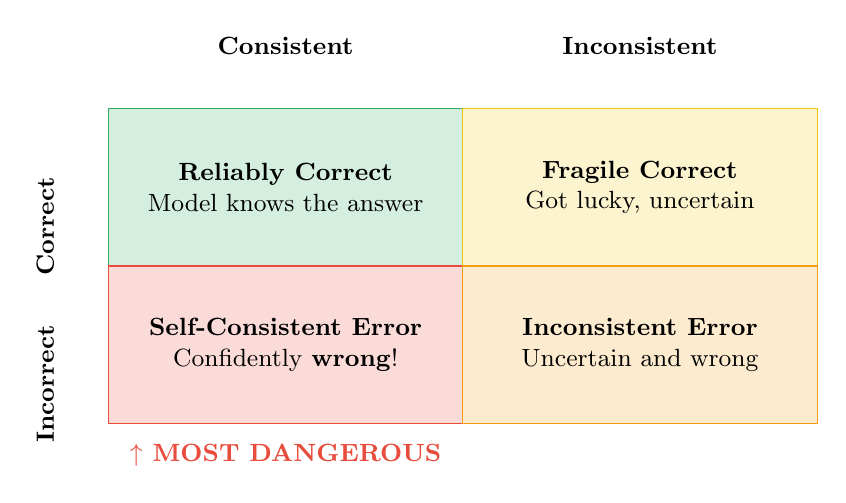
\begin{tikzpicture}[
    cell/.style={minimum width=4.5cm, minimum height=2cm, align=center, font=\small},
]
    % Headers
    \node[font=\small\bfseries] at (2.25, 3.3) {Consistent};
    \node[font=\small\bfseries] at (6.75, 3.3) {Inconsistent};
    \node[font=\small\bfseries, rotate=90] at (-0.8, 1) {Correct};
    \node[font=\small\bfseries, rotate=90] at (-0.8, -1) {Incorrect};

    % Cells
    \node[cell, fill=rcGreen!20, draw=rcGreen] at (2.25, 1.5)
        {\textbf{Reliably Correct}\\Model knows the answer};
    \node[cell, fill=fcYellow!20, draw=fcYellow] at (6.75, 1.5)
        {\textbf{Fragile Correct}\\Got lucky, uncertain};
    \node[cell, fill=ceRed!20, draw=ceRed] at (2.25, -0.5)
        {\textbf{Self-Consistent Error}\\Confidently \textbf{wrong}!};
    \node[cell, fill=ieOrange!20, draw=ieOrange] at (6.75, -0.5)
        {\textbf{Inconsistent Error}\\Uncertain and wrong};

    % Danger label
    \node[font=\small\bfseries, text=ceRed] at (2.25, -1.9) {$\uparrow$ MOST DANGEROUS};
\end{tikzpicture}
\caption{The 2$\times$2 error classification matrix. Self-consistent errors are the hardest to detect because the model shows no uncertainty signals.}
\label{fig:errormatrix}
\end{figure}

% --- Phase 1 ---
\subsection{Phase 1: Data Collection}

For each of the 807 TruthfulQA questions and each of the six models under test, I collected:
\begin{itemize}
    \item One \textbf{greedy answer} (temperature $\approx$ 0.01), representing the model's most confident response.
    \item Ten \textbf{stochastic samples} (temperature = 0.7), which probe the model's uncertainty by introducing controlled randomness.
\end{itemize}
All raw outputs were stored in JSONL format without any evaluation at this stage.

% --- Phase 2 ---
\subsection{Phase 2: Re-evaluation and Labeling}

Phase~2 processes the raw data to assign correctness and consistency labels. It does not call the model under test again; it uses local NLI and judge-side API calls.

\begin{enumerate}
    \item \textbf{Correctness evaluation.} A three-judge ensemble (OpenAI, Anthropic, xAI) with majority voting determines whether each greedy answer is correct, incorrect, or not attempted.
    \item \textbf{Semantic equivalence.} Each stochastic sample is compared to the greedy answer using a hybrid NLI approach: a local DeBERTa model handles clear cases (both directions above 0.70 $\rightarrow$ same; either below 0.30 $\rightarrow$ different), and a GPT fallback handles borderline cases.
    \item \textbf{Five-category labeling.} Based on correctness and consistency, each response is labeled as one of the five categories from Figure~\ref{fig:errormatrix}, plus \texttt{not\_attempted}. I use a primary consistency threshold of 0.9 (at least 90\% of stochastic samples must be semantically equivalent to the greedy answer for a response to count as ``consistent'').
\end{enumerate}

% --- Five-category labeling visual ---
\begin{figure}[H]
\centering
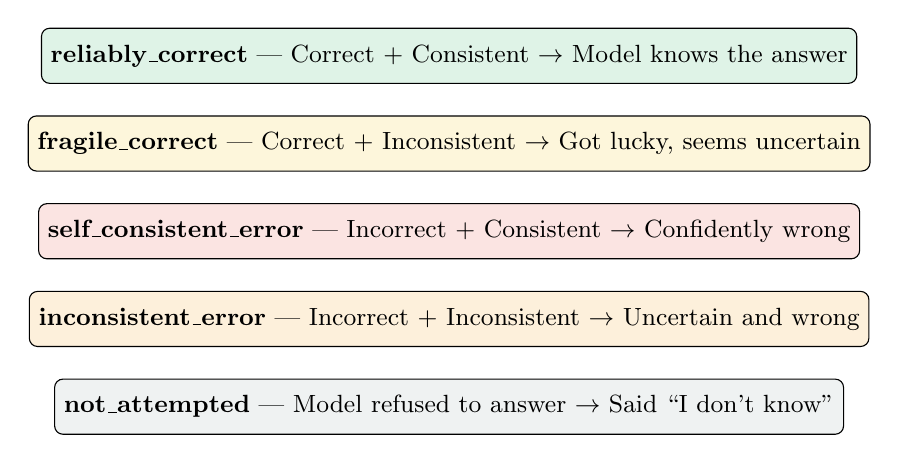
\begin{tikzpicture}[
    node distance=0.4cm,
    lbl/.style={rectangle, rounded corners=3pt, draw, minimum width=7cm, minimum height=0.7cm, align=left, font=\small},
]
    \node[lbl, fill=rcGreen!15] (rc) {\textbf{reliably\_correct} --- Correct + Consistent $\rightarrow$ Model knows the answer};
    \node[lbl, fill=fcYellow!15, below=of rc] (fc) {\textbf{fragile\_correct} --- Correct + Inconsistent $\rightarrow$ Got lucky, seems uncertain};
    \node[lbl, fill=ceRed!15, below=of fc] (ce) {\textbf{self\_consistent\_error} --- Incorrect + Consistent $\rightarrow$ Confidently wrong};
    \node[lbl, fill=ieOrange!15, below=of ce] (ie) {\textbf{inconsistent\_error} --- Incorrect + Inconsistent $\rightarrow$ Uncertain and wrong};
    \node[lbl, fill=naGray!15, below=of ie] (na) {\textbf{not\_attempted} --- Model refused to answer $\rightarrow$ Said ``I don't know''};
\end{tikzpicture}
\caption{The five-category labeling scheme applied to every (question, model) pair after Phase~2.}
\label{fig:labels}
\end{figure}

The final evaluated dataset contains 4,842 rows (807 questions $\times$ 6 models).

% --- White-Box Probe ---
\subsection{White-Box Cross-Model Probe}

This is the core detection component, adapted from Tan et al. Figure~\ref{fig:probe} shows the probe architecture, Figure~\ref{fig:fusion} shows how two probes are combined, and Figure~\ref{fig:cee2e} gives a one-page end-to-end view of the CE-only experiment.

\begin{enumerate}
    \item \textbf{Hidden state extraction.} For each question--answer pair, I run the text through two open-weight models (a response model and a verifier) and extract the hidden state vector from a selected layer. The hidden state of the last token is used, as it contains the most information about what the model is about to generate.

    \item \textbf{Probe architecture.} A small feedforward neural network (FFN) is trained on each model's hidden states. It takes a hidden state vector as input and outputs a score between 0 and 1, where higher means ``more likely to be an error.'' Training uses binary cross-entropy loss with the Phase~2 labels as ground truth.

    \item \textbf{Layer selection.} I train a separate probe per candidate layer and select the one with the highest validation AUROC.

    \item \textbf{Cross-model fusion.} The response model probe produces a score $s_M$ and the verifier probe produces $s_V$. These are fused as $s = (1 - \lambda) \cdot s_M + \lambda \cdot s_V$, with $\lambda$ selected via grid search on the validation set.

    \item \textbf{Evaluation.} AUROC, PR-AUC, accuracy at threshold 0.5, and Brier score are computed on a held-out test set (used only once).
\end{enumerate}

% --- Probe architecture diagram ---
\begin{figure}[H]
\centering
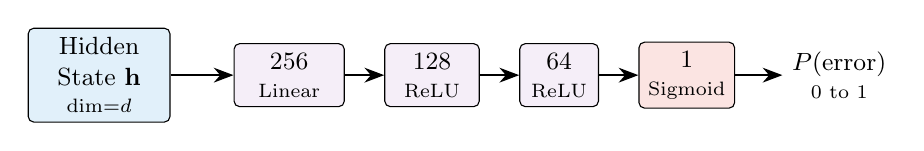
\begin{tikzpicture}[
    node distance=0.15cm,
    layer/.style={rectangle, draw, rounded corners=2pt, minimum height=0.8cm, align=center, font=\small},
    arrow/.style={-{Stealth[length=2.5mm]}, thick},
]
    \node[layer, fill=phase1Blue!15, minimum width=1.8cm] (input) {Hidden\\State $\mathbf{h}$\\[-1pt]\scriptsize dim=$d$};
    \node[layer, fill=wbPurple!10, minimum width=1.4cm, right=0.8cm of input] (l1) {256\\[-1pt]\scriptsize Linear};
    \node[layer, fill=wbPurple!10, minimum width=1.2cm, right=0.5cm of l1] (l2) {128\\[-1pt]\scriptsize ReLU};
    \node[layer, fill=wbPurple!10, minimum width=1cm, right=0.5cm of l2] (l3) {64\\[-1pt]\scriptsize ReLU};
    \node[layer, fill=ceRed!15, minimum width=0.8cm, right=0.5cm of l3] (out) {1\\[-1pt]\scriptsize Sigmoid};
    \node[right=0.6cm of out, font=\small, align=center] (plabel) {$P(\text{error})$\\[-1pt]\scriptsize 0 to 1};

    \draw[arrow] (input) -- (l1);
    \draw[arrow] (l1) -- (l2);
    \draw[arrow] (l2) -- (l3);
    \draw[arrow] (l3) -- (out);
    \draw[arrow] (out) -- (plabel);
\end{tikzpicture}
\caption{FFN probe architecture: a 4-layer feedforward network (dim $\rightarrow$ 256 $\rightarrow$ 128 $\rightarrow$ 64 $\rightarrow$ 1). The output is a probability that the answer is an error.}
\label{fig:probe}
\end{figure}

% --- Cross-model fusion diagram ---
\begin{figure}[H]
\centering
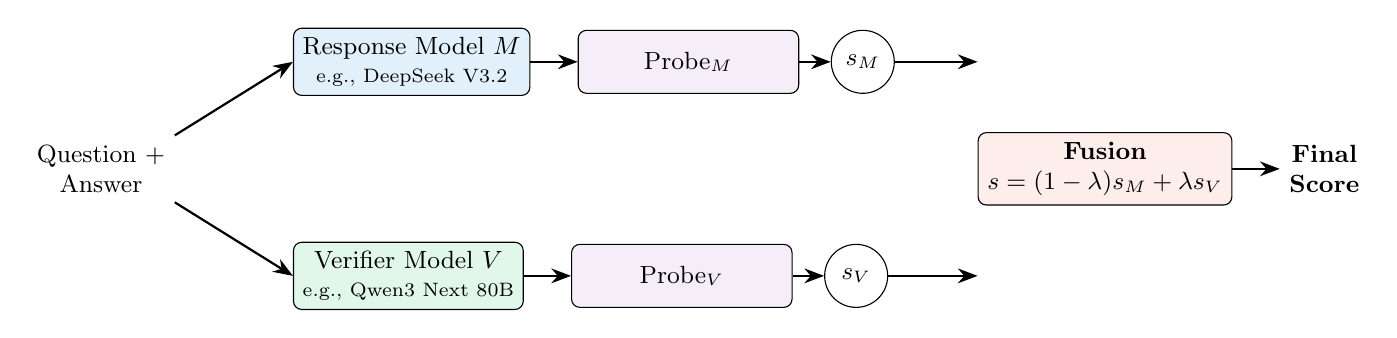
\begin{tikzpicture}[
    node distance=0.6cm and 1cm,
    box/.style={rectangle, draw, rounded corners=3pt, minimum width=2.8cm, minimum height=0.8cm, align=center, font=\small},
    score/.style={circle, draw, minimum size=0.8cm, font=\small},
    arrow/.style={-{Stealth[length=2.5mm]}, thick},
]
    % Input
    \node[font=\small, align=center] (input) {Question +\\Answer};

    % Response model
    \node[box, fill=phase1Blue!15, above right=0.5cm and 1.5cm of input] (rm) {Response Model $M$\\[-1pt]\scriptsize e.g., DeepSeek V3.2};
    \node[box, fill=wbPurple!10, right=0.6cm of rm] (pm) {Probe$_M$};
    \node[score, right=0.4cm of pm] (sm) {$s_M$};

    % Verifier model
    \node[box, fill=phase2Green!15, below right=0.5cm and 1.5cm of input] (vm) {Verifier Model $V$\\[-1pt]\scriptsize e.g., Qwen3 Next 80B};
    \node[box, fill=wbPurple!10, right=0.6cm of vm] (pv) {Probe$_V$};
    \node[score, right=0.4cm of pv] (sv) {$s_V$};

    % Fusion
    \node[box, fill=ceRed!10, right=1.5cm of $(sm)!0.5!(sv)$] (fusion) {\textbf{Fusion}\\$s = (1-\lambda)s_M + \lambda s_V$};
    \node[right=0.6cm of fusion, font=\small\bfseries, align=center] (final) {Final\\Score};

    % Arrows
    \draw[arrow] (input.north east) -- (rm.west);
    \draw[arrow] (input.south east) -- (vm.west);
    \draw[arrow] (rm) -- (pm);
    \draw[arrow] (pm) -- (sm);
    \draw[arrow] (vm) -- (pv);
    \draw[arrow] (pv) -- (sv);
    \draw[arrow] (sm.east) -- (fusion.west |- sm);
    \draw[arrow] (sv.east) -- (fusion.west |- sv);
    \draw[arrow] (fusion) -- (final);
\end{tikzpicture}
\caption{Cross-model fusion: two models, two probes, one fused score. The verifier provides a ``second opinion'' on whether the response model's answer is an error.}
\label{fig:fusion}
\end{figure}

% --- One-page CE-only end-to-end visual ---
\clearpage
\begin{figure}[p]
\centering
\resizebox{!}{0.75\textheight}{%
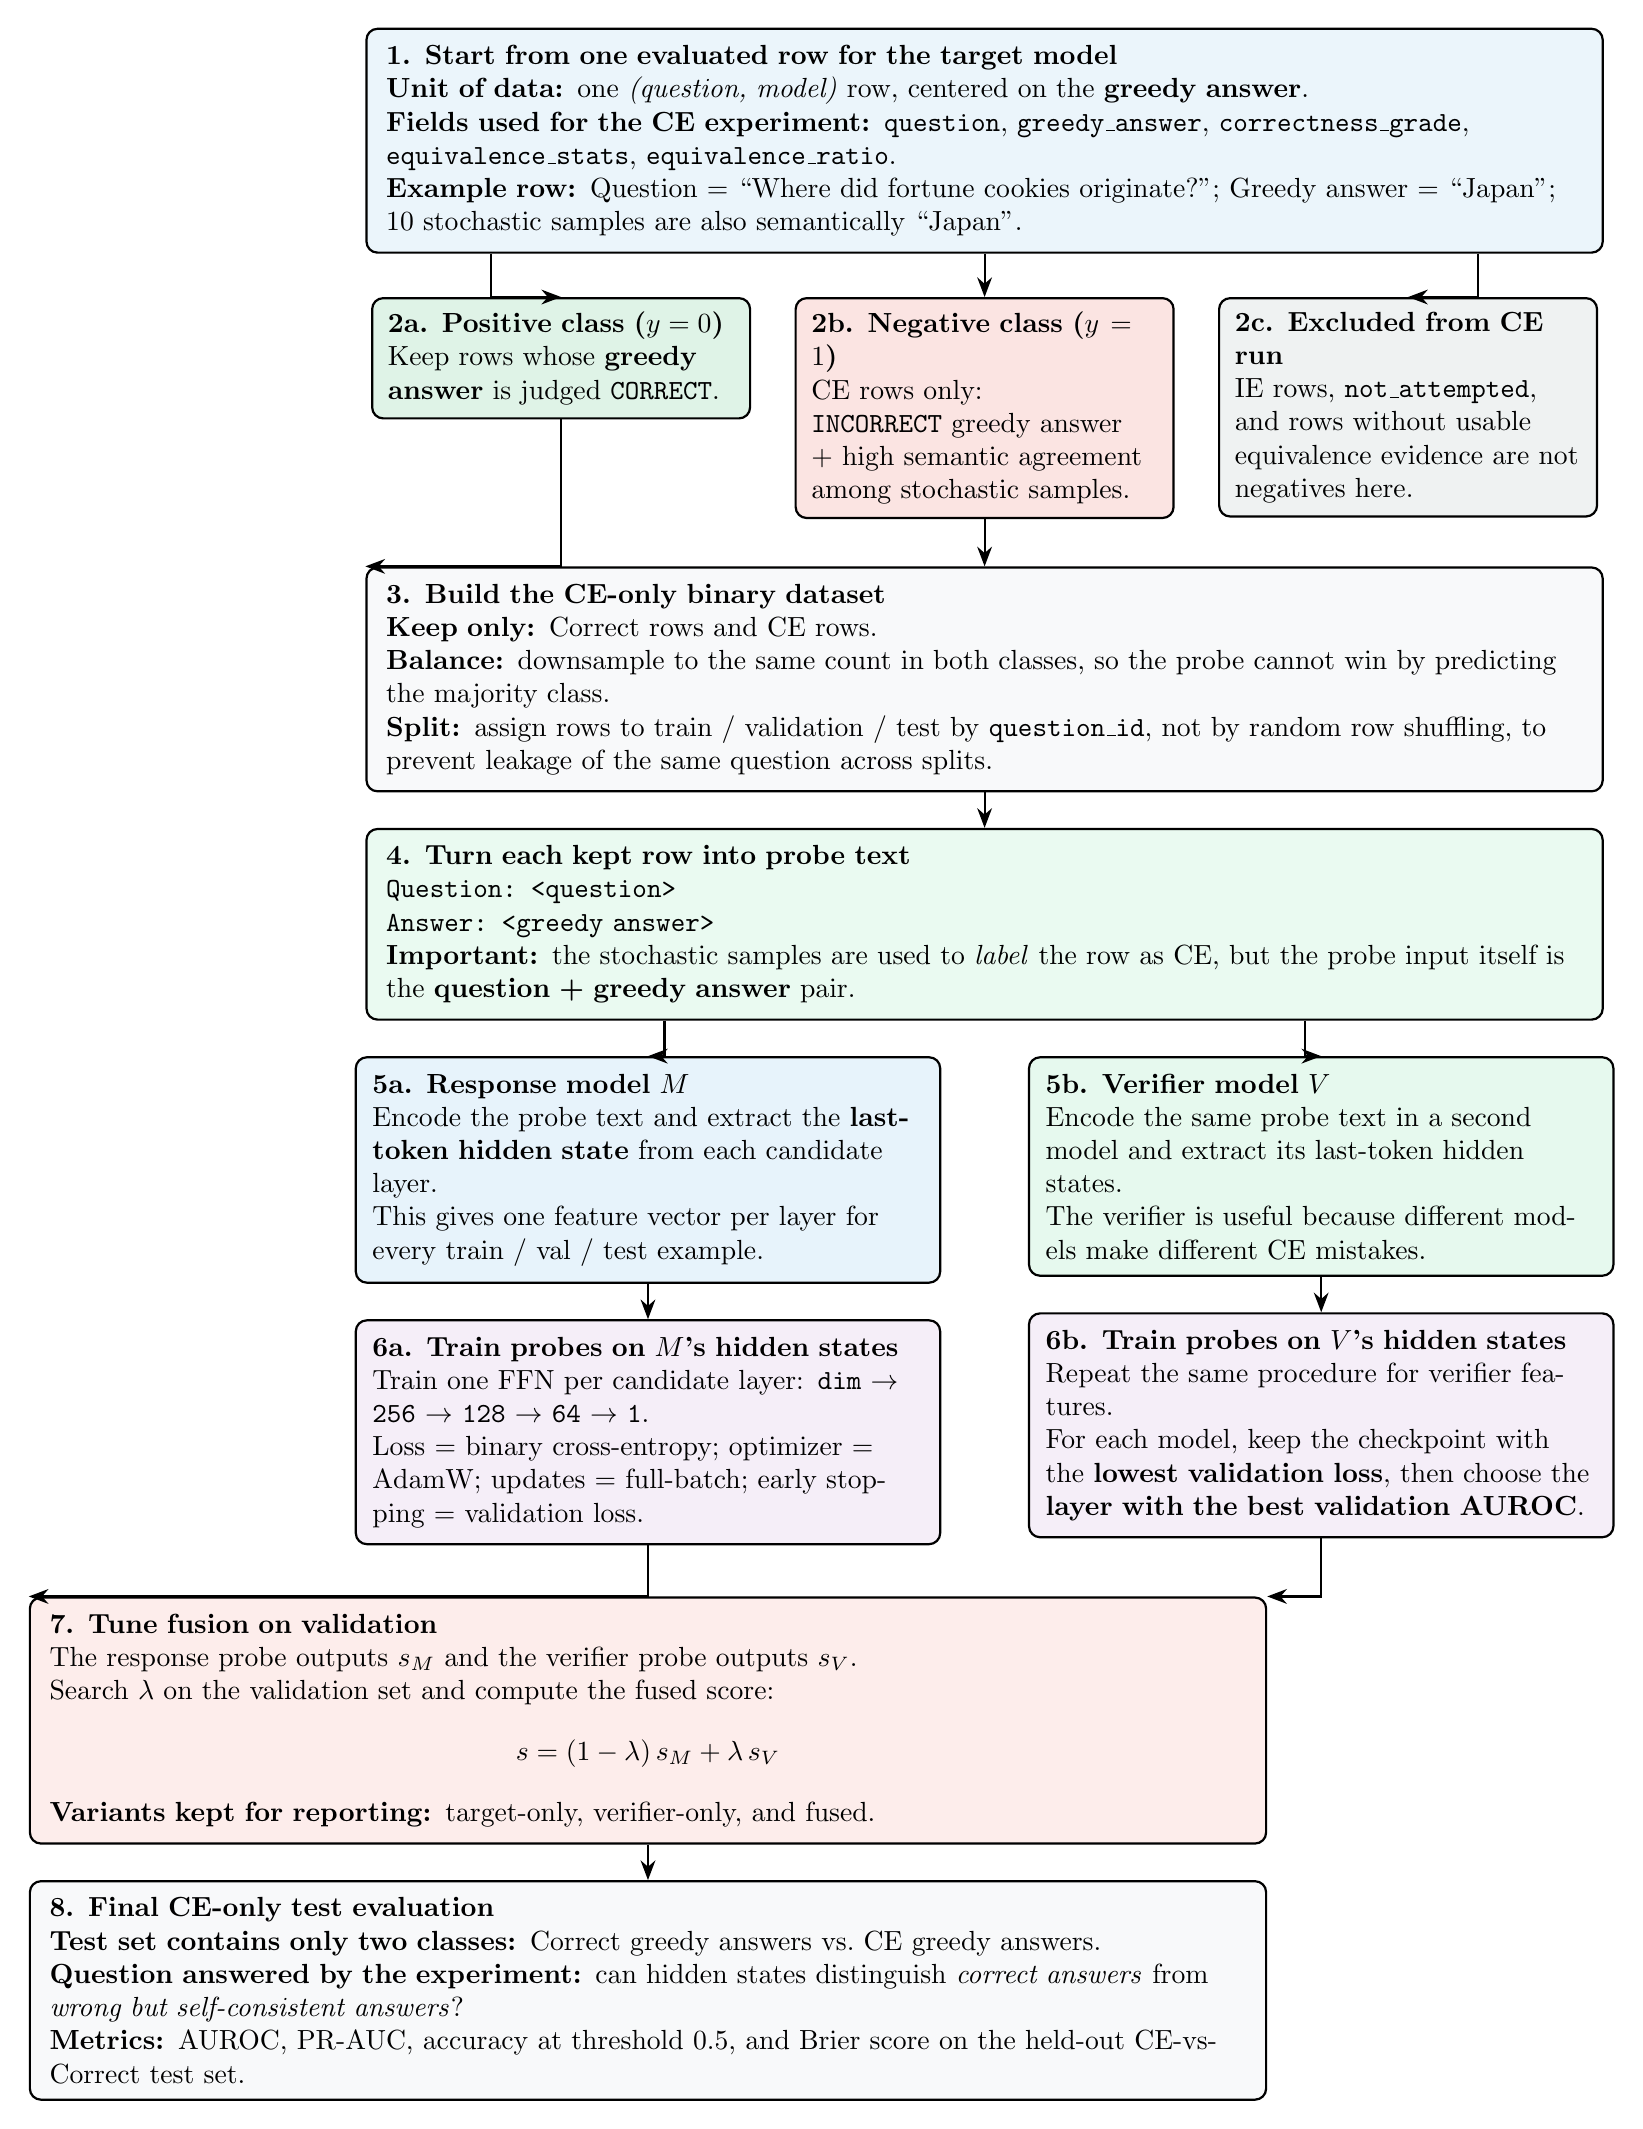
\begin{tikzpicture}[
    node distance=0.45cm and 0.55cm,
    stagebox/.style={rectangle, draw, rounded corners=4pt, thick, minimum width=15.7cm, text width=15.2cm, align=left, inner sep=6pt},
    classbox/.style={rectangle, draw, rounded corners=4pt, thick, minimum width=4.8cm, text width=4.4cm, align=left, inner sep=5pt},
    modelbox/.style={rectangle, draw, rounded corners=4pt, thick, minimum width=7.4cm, text width=7.0cm, align=left, inner sep=6pt},
    arrow/.style={-{Stealth[length=2.5mm]}, thick}
]

% Step 1
\node[stagebox, fill=phase1Blue!10] (s1) {
\textbf{1. Start from one evaluated row for the target model}\\
\textbf{Unit of data:} one \emph{(question, model)} row, centered on the \textbf{greedy answer}.\\
\textbf{Fields used for the CE experiment:} \texttt{question}, \texttt{greedy\_answer}, \texttt{correctness\_grade}, \texttt{equivalence\_stats}, \texttt{equivalence\_ratio}.\\
\textbf{Example row:} Question = ``Where did fortune cookies originate?''; Greedy answer = ``Japan''; 10 stochastic samples are also semantically ``Japan''.
};

% Step 2 label boxes
\node[classbox, fill=ceRed!15, below=0.55cm of s1.south] (c1) {
\textbf{2b. Negative class ($y=1$)}\\
CE rows only:\\
\texttt{INCORRECT} greedy answer + high semantic agreement among stochastic samples.
};
\node[classbox, fill=rcGreen!15, anchor=north east] (c0) at ([xshift=-0.55cm]c1.north west) {
\textbf{2a. Positive class ($y=0$)}\\
Keep rows whose \textbf{greedy answer} is judged \texttt{CORRECT}.
};
\node[classbox, fill=naGray!15, anchor=north west] (cx) at ([xshift=0.55cm]c1.north east) {
\textbf{2c. Excluded from CE run}\\
IE rows, \texttt{not\_attempted}, and rows without usable equivalence evidence are not negatives here.
};

\draw[arrow] (s1.south west) ++(1.6,0) |- (c0.north);
\draw[arrow] (s1.south) -- (c1.north);
\draw[arrow] (s1.south east) ++(-1.6,0) |- (cx.north);

% Step 3
\node[stagebox, fill=lightbg, below=0.6cm of c1.south] (s3) {
\textbf{3. Build the CE-only binary dataset}\\
\textbf{Keep only:} Correct rows and CE rows.\\
\textbf{Balance:} downsample to the same count in both classes, so the probe cannot win by predicting the majority class.\\
\textbf{Split:} assign rows to train / validation / test by \texttt{question\_id}, not by random row shuffling, to prevent leakage of the same question across splits.
};
\draw[arrow] (c0.south) |- (s3.north west);
\draw[arrow] (c1.south) -- (s3.north);

% Step 4
\node[stagebox, fill=phase2Green!10, below=of s3] (s4) {
\textbf{4. Turn each kept row into probe text}\\
\texttt{Question: <question>}\\
\texttt{Answer: <greedy answer>}\\
\textbf{Important:} the stochastic samples are used to \emph{label} the row as CE, but the probe input itself is the \textbf{question + greedy answer} pair.
};
\draw[arrow] (s3.south) -- (s4.north);

% Step 5 dual models
\node[modelbox, fill=phase1Blue!12, below left=of s4.south] (m1) {
\textbf{5a. Response model $M$}\\
Encode the probe text and extract the \textbf{last-token hidden state} from each candidate layer.\\
This gives one feature vector per layer for every train / val / test example.
};
\node[modelbox, fill=phase2Green!12, below right=of s4.south] (m2) {
\textbf{5b. Verifier model $V$}\\
Encode the same probe text in a second model and extract its last-token hidden states.\\
The verifier is useful because different models make different CE mistakes.
};
\draw[arrow] (s4.south west) ++(3.8,0) |- (m1.north);
\draw[arrow] (s4.south east) ++(-3.8,0) |- (m2.north);

% Step 6 probes
\node[modelbox, fill=wbPurple!10, below=of m1] (p1) {
\textbf{6a. Train probes on $M$'s hidden states}\\
Train one FFN per candidate layer: \texttt{dim $\rightarrow$ 256 $\rightarrow$ 128 $\rightarrow$ 64 $\rightarrow$ 1}.\\
Loss = binary cross-entropy; optimizer = AdamW; updates = full-batch; early stopping = validation loss.
};
\node[modelbox, fill=wbPurple!10, below=of m2] (p2) {
\textbf{6b. Train probes on $V$'s hidden states}\\
Repeat the same procedure for verifier features.\\
For each model, keep the checkpoint with the \textbf{lowest validation loss}, then choose the \textbf{layer with the best validation AUROC}.
};
\draw[arrow] (m1.south) -- (p1.north);
\draw[arrow] (m2.south) -- (p2.north);

% Step 7
\node[stagebox, fill=ceRed!10, below=0.65cm of p1.south] (s7) {
\textbf{7. Tune fusion on validation}\\
The response probe outputs $s_M$ and the verifier probe outputs $s_V$.\\
Search $\lambda$ on the validation set and compute the fused score:
\[
s = (1-\lambda)\, s_M + \lambda\, s_V
\]
\textbf{Variants kept for reporting:} target-only, verifier-only, and fused.
};
\draw[arrow] (p1.south) |- (s7.north west);
\draw[arrow] (p2.south) |- (s7.north east);

% Step 8
\node[stagebox, fill=lightbg, below=of s7] (s8) {
\textbf{8. Final CE-only test evaluation}\\
\textbf{Test set contains only two classes:} Correct greedy answers vs.\ CE greedy answers.\\
\textbf{Question answered by the experiment:} can hidden states distinguish \emph{correct answers} from \emph{wrong but self-consistent answers}?\\
\textbf{Metrics:} AUROC, PR-AUC, accuracy at threshold 0.5, and Brier score on the held-out CE-vs-Correct test set.
};
\draw[arrow] (s7.south) -- (s8.north);

\end{tikzpicture}
}
\caption{One-page end-to-end view of the CE-only cross-model probing experiment. The task is binary: \textbf{Correct} vs.\ \textbf{Self-Consistent Error (CE)}. The stochastic samples define the CE label, while the probe itself sees only the question and the greedy answer.}
\label{fig:cee2e}
\end{figure}
\clearpage

\paragraph{How I read Figure~\ref{fig:cee2e} in practice.}
\begin{itemize}
    \item Suppose I use DeepSeek V3.2 as the response model $M$ and Qwen3 Next 80B as the verifier $V$.
    \item If the question is ``Where did fortune cookies originate?'' and DeepSeek's greedy answer is ``Japan,'' then this row becomes a CE example only if the greedy answer is judged \texttt{INCORRECT} and the sampled answers are also semantically ``Japan.'' In that case, I assign $y=1$.
    \item A row such as ``What is the capital of France?'' $\rightarrow$ ``Paris'' becomes a correct example and gets $y=0$.
    \item I keep only \textbf{Correct} and \textbf{CE} on purpose. CE is the hard case I care about: the answer is wrong, but it still looks stable and confident. If I mixed IE rows into the same task, the probe could partly win by learning uncertainty instead of learning the harder boundary between \emph{right} and \emph{wrong but self-consistent}.
    \item After labeling, I balance the two classes and split by \texttt{question\_id} so the same question cannot leak across train, validation, and test.
    \item I then turn each retained row into \texttt{Question: ... Answer: ...}. I use both because correctness depends on the question, not on the answer string alone.
    \item I run that same text through both models, extract the last-token hidden state from candidate layers, and train a small FFN probe on top of each layer. I do this separately for DeepSeek features and Qwen features because the two models may encode CE errors differently.
    \item On validation, I keep the checkpoint with the lowest validation loss, choose the layer with the best validation AUROC, and tune the fusion weight $\lambda$.
    \item On the held-out test set, the question is very narrow: can these hidden states distinguish \emph{correct answers} from \emph{wrong but self-consistent answers}?
\end{itemize}

\subsection{What Hidden States Seem to Carry (Research View)}

Research does \emph{not} show one simple visual pattern like ``a hallucination neuron.'' Instead, hidden states act as high-dimensional representations where truth-related signals can often be extracted by small probes.

\begin{itemize}
    \item \textbf{Truthfulness is probe-readable from activations.} Azaria and Mitchell show that classifiers trained on hidden activations can predict true vs.\ false statements, and they explicitly compare this against sentence probability baselines.\footnote{A. Azaria and T. Mitchell, \emph{The Internal State of an LLM Knows When It's Lying}, Findings of EMNLP 2023. \href{https://aclanthology.org/2023.findings-emnlp.68/}{ACL Anthology}.}
    \item \textbf{Self-consistent errors are especially hard for output-side detectors.} Tan et al.\ define CE formally and show that mainstream detectors struggle, motivating cross-model fusion of hidden-state evidence.\footnote{H. Tan et al., \emph{Too Consistent to Detect: A Study of Self-Consistent Errors in LLMs}, EMNLP 2025. \href{https://aclanthology.org/2025.emnlp-main.238/}{ACL Anthology}.}
    \item \textbf{Hidden states are strongly predictive of factuality in long-form generation.} Han et al.\ show lightweight probes on hidden states can be competitive with expensive multi-sample detectors, with large compute savings.\footnote{J. Han et al., \emph{Simple Factuality Probes Detect Hallucinations in Long-Form Natural Language Generation}, Findings of EMNLP 2025. \href{https://aclanthology.org/2025.findings-emnlp.880/}{ACL Anthology}.}
    \item \textbf{Hidden states also encode semantic uncertainty signals.} Farquhar et al.\ motivate uncertainty at the \emph{meaning} level (semantic entropy), and Kossen et al.\ show this uncertainty can be approximated directly from hidden states using probes.\footnote{S. Farquhar et al., \emph{Detecting hallucinations in large language models using semantic entropy}, Nature 2024. \href{https://doi.org/10.1038/s41586-024-07421-0}{DOI}. J. Kossen et al., \emph{Semantic Entropy Probes: Robust and Cheap Hallucination Detection in LLMs}, arXiv 2024. \href{https://arxiv.org/abs/2406.15927}{arXiv}.}
\end{itemize}

So in practical terms: correct answers and CE answers tend to occupy different but partially overlapping regions of activation space; the CE boundary is subtler than easy uncertainty cases, which is why a trained probe (and often cross-model fusion) helps.

\subsection{Why Softmax Alone Is Not Enough}

Softmax gives a distribution over the \emph{next token}, not a direct estimate of ``this full answer is factually correct.'' For CE, this matters:
\begin{itemize}
    \item A model can assign high probability to fluent but wrong continuations, so token confidence can be high while factuality is low.
    \item Sentence/token probabilities are confounded by factors like length and word frequency, which Azaria and Mitchell explicitly analyze.
    \item Token-level uncertainty misses paraphrase effects (different strings, same meaning). Semantic entropy work shows meaning-level uncertainty is more reliable for hallucination risk.
    \item CE examples are often confidently wrong by definition, so output-side confidence alone can look ``certain'' even when the answer is false.
\end{itemize}

That is why this pipeline uses hidden-state probes (plus verifier fusion) instead of relying on softmax confidence alone.

I used the three open-weight models from my black-box evaluation---DeepSeek V3.2, Qwen3 Next 80B, and Llama 4 Maverick 17B---for white-box probing, since they are the only ones that expose hidden states. Table~\ref{tab:pairings} shows the cross-model pairings.

\begin{table}[H]
\centering
\begin{tabular}{lll}
\toprule
\textbf{Response Model} & \textbf{Verifier Option 1} & \textbf{Verifier Option 2} \\
\midrule
DeepSeek V3.2 & Qwen3 Next 80B & Llama 4 Maverick 17B \\
Qwen3 Next 80B & DeepSeek V3.2 & Llama 4 Maverick 17B \\
Llama 4 Maverick 17B & DeepSeek V3.2 & Qwen3 Next 80B \\
\bottomrule
\end{tabular}
\caption{Cross-model probe pairings. Each response model is paired with two verifiers from different model families.}
\label{tab:pairings}
\end{table}

\subsection{Key Design Choices}

\begin{itemize}
    \item \textbf{Question-level data splits.} Train/validation/test splits are done at the question level (80/10/10) to prevent data leakage. A fixed split seed ensures reproducibility.
    \item \textbf{Z-score normalization.} Hidden state features are standardized using the training set mean and standard deviation before probe training.
    \item \textbf{Early stopping.} Training runs for up to 300 epochs with patience of 25. If validation performance stops improving, training stops early to prevent overfitting.
    \item \textbf{Multiple seeds.} Probes are trained with multiple random seeds, and I report mean $\pm$ std of metrics to confirm stability.
\end{itemize}

% ============================================================
\section{Differences from the Original Paper}
% ============================================================

My implementation is faithful to Tan et al., with a few documented differences:

\begin{table}[H]
\centering
\begin{tabular}{lll}
\toprule
\textbf{Aspect} & \textbf{Tan et al.} & \textbf{My Implementation} \\
\midrule
Dataset & TriviaQA, SciQ & TruthfulQA (807 questions) \\
Normalization & None reported & Z-score normalization \\
Response models & Direct model access & API-based with local encoder proxies \\
\bottomrule
\end{tabular}
\caption{Documented differences from the original paper.}
\end{table}

These differences are acceptable because TruthfulQA is specifically designed for hallucination research, Z-score normalization is standard practice, and local encoder proxies are necessary when some response models are only available through APIs.

% ============================================================
\section{Results}
% ============================================================

\subsection{Black-Box Results: Self-Consistent Error Rates}

Table~\ref{tab:cerates} presents the self-consistent error rates from my black-box pipeline across all six models (threshold 0.9). Figure~\ref{fig:cebar} visualizes the CE rate and CE share of errors.

\begin{table}[H]
\centering
\begin{tabular}{lrrrr}
\toprule
\textbf{Model} & \textbf{Accuracy} & \textbf{CE Count} & \textbf{CE Rate} & \textbf{CE \% of Errors} \\
\midrule
Claude Opus 4.6     & 74.7\% & 100 & 12.4\% & 59.2\% \\
Qwen3 Next 80B      & 65.2\% & 162 & 20.1\% & 65.6\% \\
DeepSeek V3.2        & 60.3\% & 168 & 20.8\% & 60.9\% \\
GPT-5.2              & 69.8\% &  79 &  9.8\% & 36.4\% \\
Grok 4               & 57.1\% & 106 & 13.1\% & 33.1\% \\
Llama 4 Maverick 17B & 52.4\% & 148 & 18.3\% & 44.7\% \\
\midrule
\textbf{Overall}     & 63.3\% & 763 & 13.5\% & 48.9\% \\
\bottomrule
\end{tabular}
\caption{Self-consistent error rates across models at threshold 0.9. CE Rate = percentage of all questions. CE \% of Errors = percentage of incorrect answers that are self-consistent.}
\label{tab:cerates}
\end{table}

% --- Bar chart for CE rates ---
\begin{figure}[H]
\centering
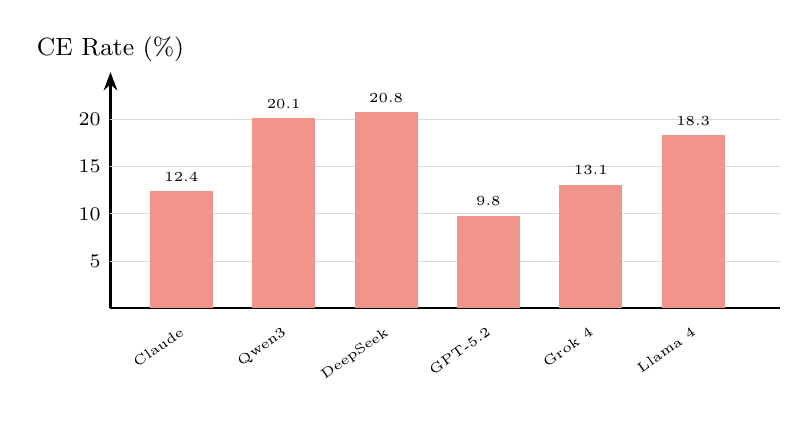
\begin{tikzpicture}[yscale=0.12, xscale=1]
    % Axes
    \draw[thick, -{Stealth}] (0,0) -- (0, 25) node[above, font=\small] {CE Rate (\%)};
    \draw[thick] (0,0) -- (8.5,0);

    % Grid lines
    \foreach \y in {5,10,15,20} {
        \draw[gray!30] (0,\y) -- (8.5,\y);
        \node[left, font=\scriptsize] at (0,\y) {\y};
    }

    % Bars
    \fill[ceRed!60] (0.5,0) rectangle (1.3, 12.4);
    \fill[ceRed!60] (1.8,0) rectangle (2.6, 20.1);
    \fill[ceRed!60] (3.1,0) rectangle (3.9, 20.8);
    \fill[ceRed!60] (4.4,0) rectangle (5.2, 9.8);
    \fill[ceRed!60] (5.7,0) rectangle (6.5, 13.1);
    \fill[ceRed!60] (7.0,0) rectangle (7.8, 18.3);

    % Labels
    \node[below, font=\tiny, rotate=35, anchor=north east] at (0.9, -0.5) {Claude};
    \node[below, font=\tiny, rotate=35, anchor=north east] at (2.2, -0.5) {Qwen3};
    \node[below, font=\tiny, rotate=35, anchor=north east] at (3.5, -0.5) {DeepSeek};
    \node[below, font=\tiny, rotate=35, anchor=north east] at (4.8, -0.5) {GPT-5.2};
    \node[below, font=\tiny, rotate=35, anchor=north east] at (6.1, -0.5) {Grok 4};
    \node[below, font=\tiny, rotate=35, anchor=north east] at (7.4, -0.5) {Llama 4};

    % Value labels
    \node[above, font=\tiny] at (0.9, 12.4) {12.4};
    \node[above, font=\tiny] at (2.2, 20.1) {20.1};
    \node[above, font=\tiny] at (3.5, 20.8) {20.8};
    \node[above, font=\tiny] at (4.8, 9.8) {9.8};
    \node[above, font=\tiny] at (6.1, 13.1) {13.1};
    \node[above, font=\tiny] at (7.4, 18.3) {18.3};
\end{tikzpicture}
\caption{Self-consistent error rate (\%) by model at threshold 0.9. Higher accuracy does not guarantee a lower CE rate.}
\label{fig:cebar}
\end{figure}

Key observations:
\begin{itemize}
    \item Self-consistent errors are \textbf{common}: 10--21\% of questions result in CEs depending on the model.
    \item Higher accuracy does \textbf{not} guarantee fewer CEs: Claude has the highest accuracy (74.7\%) but still has a 12.4\% CE rate.
    \item Among errors, \textbf{33--66\% are self-consistent}---a substantial share that shows no uncertainty signal.
    \item The overall CE rate across all 4,842 rows is 13.5\%, with CEs making up 48.9\% of all incorrect answers.
\end{itemize}

\subsection{Black-Box Results: Cross-Model CE Overlap}

A critical finding that motivates the cross-model probe: self-consistent errors \textbf{rarely overlap} across models. Table~\ref{tab:overlap} shows this for the open-weight model pairs used in the white-box probe.

\begin{table}[H]
\centering
\begin{tabular}{llrrrr}
\toprule
\textbf{Model A} & \textbf{Model B} & \textbf{A CEs} & \textbf{B CEs} & \textbf{Overlap} & \textbf{Jaccard} \\
\midrule
DeepSeek V3.2   & Qwen3 Next 80B      & 168 & 162 & 86 & 0.352 \\
DeepSeek V3.2   & Llama 4 Maverick     & 168 & 148 & 83 & 0.356 \\
Llama 4 Mav.    & Qwen3 Next 80B       & 148 & 162 & 79 & 0.342 \\
\bottomrule
\end{tabular}
\caption{Pairwise CE overlap for the three open-weight model pairs used in white-box probing. Jaccard similarity is below 36\% in all cases, confirming that models make different self-consistent errors.}
\label{tab:overlap}
\end{table}

% --- Jaccard visual ---
\begin{figure}[H]
\centering
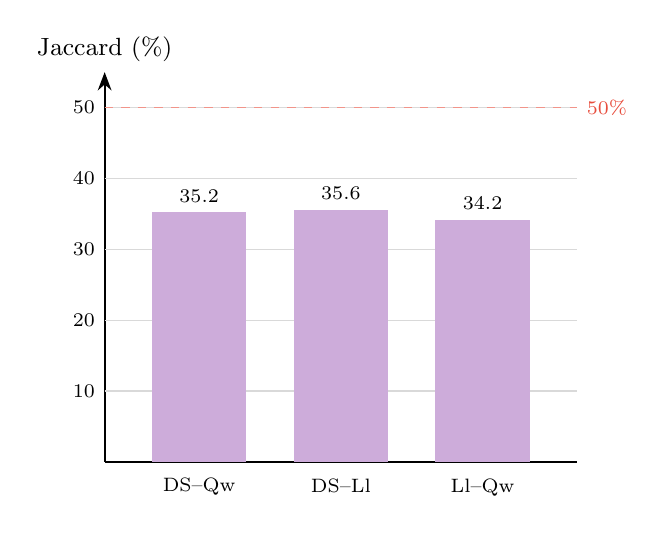
\begin{tikzpicture}[yscale=0.09, xscale=1.2]
    % Axes
    \draw[thick, -{Stealth}] (0,0) -- (0, 55) node[above, font=\small] {Jaccard (\%)};
    \draw[thick] (0,0) -- (5,0);

    % Grid
    \foreach \y in {10,20,30,40,50} {
        \draw[gray!30] (0,\y) -- (5,\y);
        \node[left, font=\scriptsize] at (0,\y) {\y};
    }

    % 50% line
    \draw[dashed, ceRed!60] (0,50) -- (5,50);
    \node[right, font=\scriptsize, text=ceRed] at (5, 50) {50\%};

    % Bars
    \fill[wbPurple!50] (0.5,0) rectangle (1.5, 35.2);
    \fill[wbPurple!50] (2.0,0) rectangle (3.0, 35.6);
    \fill[wbPurple!50] (3.5,0) rectangle (4.5, 34.2);

    % Labels
    \node[below, font=\scriptsize, align=center] at (1.0, -1) {DS--Qw};
    \node[below, font=\scriptsize, align=center] at (2.5, -1) {DS--Ll};
    \node[below, font=\scriptsize, align=center] at (4.0, -1) {Ll--Qw};

    % Values
    \node[above, font=\scriptsize] at (1.0, 35.2) {35.2};
    \node[above, font=\scriptsize] at (2.5, 35.6) {35.6};
    \node[above, font=\scriptsize] at (4.0, 34.2) {34.2};
\end{tikzpicture}
\caption{Jaccard similarity of CE sets between model pairs. All values are well below 50\%, meaning the models make different self-consistent errors---exactly the condition needed for cross-model probing to work.}
\label{fig:jaccard}
\end{figure}

The low Jaccard overlap (34--36\%) means that when Model A makes a self-consistent error, Model B usually does \emph{not} make the same error. This is consistent with Tan et al.'s findings (5--29\% overlap on TriviaQA/SciQ) and validates the cross-model approach.

\subsection{Black-Box Baseline: Why Consistency Detectors Fail on CEs}

Before the white-box probe, I also evaluated two standard black-box detectors---disagreement probability and semantic entropy---as baselines. These are consistency-based methods that detect errors by looking for variation across stochastic samples.

\begin{table}[H]
\centering
\begin{tabular}{lcccc}
\toprule
\textbf{Detector} & \textbf{AUROC} & \textbf{PR-AUC} & \textbf{Acc@0.5} & \textbf{Brier} \\
\midrule
Disagreement Probability & 0.560 & 0.393 & 0.605 & 0.314 \\
Semantic Entropy         & 0.575 & 0.411 & 0.639 & 0.285 \\
\bottomrule
\end{tabular}
\caption{Black-box detector performance on all answered rows (4,623). Both methods perform barely above random guessing (AUROC 0.5), confirming that consistency-based detectors cannot reliably catch CEs.}
\label{tab:bbbaseline}
\end{table}

% --- Visual: AUROC comparison ---
\begin{figure}[H]
\centering
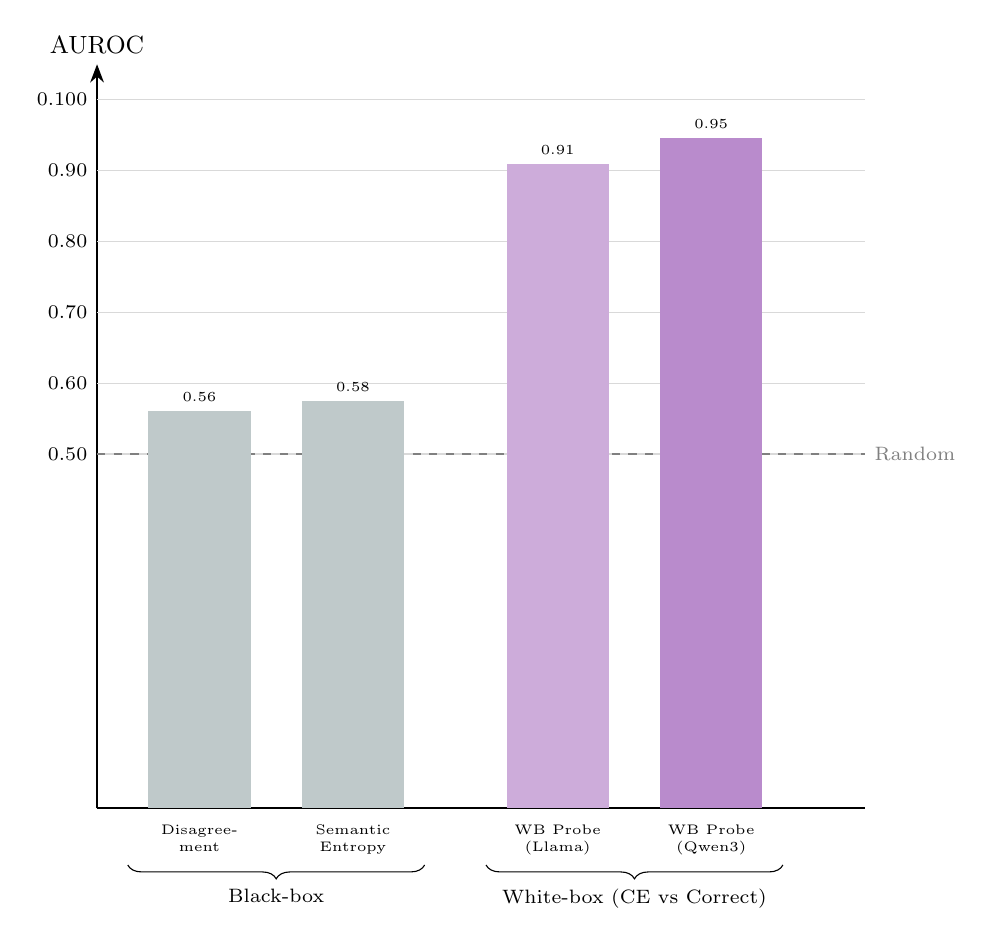
\begin{tikzpicture}[yscale=0.09, xscale=1.3]
    % Axes
    \draw[thick, -{Stealth}] (0,0) -- (0, 105) node[above, font=\small] {AUROC};
    \draw[thick] (0,0) -- (7.5,0);

    % Grid
    \foreach \y in {50, 60, 70, 80, 90, 100} {
        \draw[gray!30] (0,\y) -- (7.5,\y);
        \node[left, font=\scriptsize] at (0,\y) {0.\y};
    }

    % Random line
    \draw[dashed, gray] (0,50) -- (7.5,50);
    \node[right, font=\scriptsize, text=gray] at (7.5, 50) {Random};

    % Black-box bars
    \fill[naGray!60] (0.5,0) rectangle (1.5, 56.0);
    \fill[naGray!60] (2.0,0) rectangle (3.0, 57.5);

    % White-box bars (CE vs Correct) -- best Nibi results
    \fill[wbPurple!50] (4.0,0) rectangle (5.0, 90.9);
    \fill[wbPurple!70] (5.5,0) rectangle (6.5, 94.6);

    % Labels
    \node[below, font=\tiny, align=center] at (1.0, -1) {Disagree-\\ment};
    \node[below, font=\tiny, align=center] at (2.5, -1) {Semantic\\Entropy};
    \node[below, font=\tiny, align=center] at (4.5, -1) {WB Probe\\(Llama)};
    \node[below, font=\tiny, align=center] at (6.0, -1) {WB Probe\\(Qwen3)};

    % Values
    \node[above, font=\tiny] at (1.0, 56.0) {0.56};
    \node[above, font=\tiny] at (2.5, 57.5) {0.58};
    \node[above, font=\tiny] at (4.5, 90.9) {0.91};
    \node[above, font=\tiny] at (6.0, 94.6) {0.95};

    % Group labels
    \draw[decorate, decoration={brace, amplitude=5pt, mirror}] (0.3,-8) -- (3.2,-8)
        node[midway, below=5pt, font=\scriptsize] {Black-box};
    \draw[decorate, decoration={brace, amplitude=5pt, mirror}] (3.8,-8) -- (6.7,-8)
        node[midway, below=5pt, font=\scriptsize] {White-box (CE vs Correct)};
\end{tikzpicture}
\caption{AUROC comparison: black-box consistency detectors vs.\ white-box probes for detecting self-consistent errors. The white-box probes dramatically outperform the black-box baselines.}
\label{fig:auroccompare}
\end{figure}

Both black-box detectors achieve AUROC barely above 0.5 (random guessing). This confirms Tan et al.'s core finding: consistency-based methods fundamentally cannot detect CEs because CEs show no variation across samples. This is exactly the gap the white-box probe is designed to fill.

\subsection{White-Box Probe Results (Nibi HPC Cluster)}

I re-synced Nibi outputs on March 15, 2026 and re-evaluated the currently available runs. At snapshot time, \texttt{squeue -u ssimran5} showed one active non-report job (\texttt{qwen807}, JobID 10408307), while white-box artifacts for completed runs were already present on \texttt{\$SCRATCH}. The synced artifacts include:
\begin{itemize}
    \item six completed runs for all six target models with fixed encoders: response proxy \texttt{HuggingFaceTB/SmolLM3-3B} and verifier \texttt{microsoft/Phi-4-mini-instruct};
    \item six completed all-target reruns with response proxy \texttt{Qwen/Qwen3.5-4B} and verifier \texttt{microsoft/Phi-4-mini-instruct};
    \item five preserved historical response=target runs from \texttt{wb\_probe\_out};
\end{itemize}
All results below use three probe seeds (11, 22, 33), CE threshold 1.0, and report mean $\pm$ std across seeds.

\paragraph{Why this fixed setup (\texttt{SmolLM3-3B + Phi-4-mini})?}
The response models in my benchmark are API models, so I cannot directly read their hidden states. I therefore use a fixed local response proxy and a fixed verifier for all targets. This makes the white-box comparison controlled: the encoder stack is constant, and only the target model's error distribution changes. In other words, this is a deliberate cross-model proxy experiment (not a strict ``response=target'' replay), designed to test whether internal-state signals generalize across closed-model targets.

\begin{table}[H]
\centering
\small
\begin{tabular}{lll}
\toprule
\textbf{Run Group} & \textbf{Targets Covered} & \textbf{Status} \\
\midrule
\texttt{SmolLM3-3B + Phi-4-mini} & 6/6 targets & Completed (metrics present) \\
\texttt{Qwen3.5-4B + Phi-4-mini} & 6/6 targets & Completed (metrics present) \\
\bottomrule
\end{tabular}
\caption{Nibi run inventory after the March 15, 2026 live sync.}
\label{tab:nibi_runs}
\end{table}

\subsubsection{Local Sync Inventory (March 15, 2026)}

I copied all completed Nibi white-box artifacts into:
\texttt{data/results/whitebox/nibi\_sync\_2026-03-15/live\_pull/}
with a machine-readable manifest at:
\texttt{.../live\_pull/manifests/sync\_manifest.csv}.

\begin{table}[H]
\centering
\small
\begin{tabular}{lccc}
\toprule
\textbf{Local Mirror Subfolder} & \textbf{Run Dirs} & \textbf{Unique (Target,Resp,Ver)} & \textbf{Notes} \\
\midrule
\texttt{smollm3\_phi\_base} & 6 & 6 & all 6 targets \\
\texttt{qwen35\_phi\_all6} & 6 & 6 & all 6 targets \\
\texttt{legacy\_wb\_probe\_out} & 5 & 5 & preserved response=target runs \\
\midrule
\textbf{Total} & \textbf{17} & \textbf{17} & no duplicate config in this report scope \\
\bottomrule
\end{tabular}
\caption{Local synced inventory after copying all completed Nibi result folders.}
\label{tab:nibi_local_sync_inventory}
\end{table}

\begin{table}[H]
\centering
\scriptsize
\resizebox{\textwidth}{!}{%
\begin{tabular}{lccr}
\toprule
\textbf{Response Proxy} & \textbf{Verifier} & \textbf{Unique Target Models} & \textbf{Run Dirs} \\
\midrule
\texttt{HuggingFaceTB/SmolLM3-3B} & \texttt{microsoft/Phi-4-mini-instruct} & 6 & 6 \\
\texttt{Qwen/Qwen3.5-4B} & \texttt{microsoft/Phi-4-mini-instruct} & 6 & 6 \\
\texttt{meta-llama/Llama-4-Maverick-17B-128E-Instruct} & \texttt{meta-llama/Llama-3.1-8B-Instruct} & 1 & 1 \\
\texttt{meta-llama/Llama-4-Maverick-17B-128E-Instruct} & \texttt{Qwen/Qwen2.5-0.5B-Instruct} & 1 & 1 \\
\texttt{meta-llama/Llama-4-Maverick-17B-128E-Instruct} & \texttt{Qwen/Qwen3-Next-80B-A3B-Instruct} & 1 & 1 \\
\texttt{Qwen/Qwen3-Next-80B-A3B-Instruct} & \texttt{meta-llama/Llama-3.1-8B-Instruct} & 1 & 1 \\
\texttt{Qwen/Qwen3-Next-80B-A3B-Instruct} & \texttt{Qwen/Qwen2.5-0.5B-Instruct} & 1 & 1 \\
\bottomrule
\end{tabular}
}
\caption{Run-group coverage in the local mirror.}
\label{tab:nibi_local_sync_groups}
\end{table}

\subsubsection{Run-Group CE Metrics (Three Groups)}

The following CE tables report target-only AUROC, verifier-only AUROC, fused AUROC, and fused $\lambda$. Best variant per target is shown in bold (ties are bolded in all tied columns).

\paragraph{Setup (\texttt{smollm3\_phi\_base})}
Response model = \texttt{SmolLM3-3B}, verifier model = \texttt{Phi-4-mini-instruct}.
\begin{table}[H]
\centering
\scriptsize
\resizebox{\textwidth}{!}{%
\begin{tabular}{lrrrrrrrrr}
\toprule
\textbf{Target Model} & \textbf{Target AUROC} & \textbf{Verifier AUROC} & \textbf{Fused AUROC} & \textbf{Fused $\lambda$} & \textbf{CE Pool (C/CE)} & \textbf{Train (C/CE)} & \textbf{Val (C/CE)} & \textbf{Test (C/CE)} & \textbf{Test N} \\
\midrule
Claude Opus 4.6 & 0.9519 & \textbf{1.0000} & 0.9852 & 0.2667 & 90/90 & 72/73 & 3/11 & 15/6 & 21 \\
DeepSeek V3.2 & 0.8516 & \textbf{0.8776} & 0.8750 & 0.9667 & 143/143 & 125/116 & 10/11 & 8/16 & 24 \\
GPT-5.2 & 0.9352 & \textbf{0.9722} & 0.9352 & 0.0000 & 61/61 & 51/48 & 4/7 & 6/6 & 12 \\
Grok 4 & 0.9231 & \textbf{0.9487} & 0.9231 & 0.0000 & 88/88 & 81/67 & 4/8 & 3/13 & 16 \\
Llama 4 Maverick 17B & \textbf{0.8775} & 0.8575 & \textbf{0.8775} & 0.0000 & 125/125 & 106/103 & 10/9 & 9/13 & 22 \\
Qwen3 Next 80B & \textbf{0.9152} & 0.8839 & 0.9137 & 0.4500 & 146/146 & 120/120 & 10/12 & 16/14 & 30 \\
\bottomrule
\end{tabular}
}
\caption{CE metrics for run group \texttt{smollm3\_phi\_base}.}
\label{tab:group_smollm3_phi_base_ce}
\end{table}

\paragraph{Setup (\texttt{qwen35\_phi\_all6})}
Response model = \texttt{Qwen3.5-4B}, verifier model = \texttt{Phi-4-mini-instruct}.
\begin{table}[H]
\centering
\scriptsize
\resizebox{\textwidth}{!}{%
\begin{tabular}{lrrrrrrrrr}
\toprule
\textbf{Target Model} & \textbf{Target AUROC} & \textbf{Verifier AUROC} & \textbf{Fused AUROC} & \textbf{Fused $\lambda$} & \textbf{CE Pool (C/CE)} & \textbf{Train (C/CE)} & \textbf{Val (C/CE)} & \textbf{Test (C/CE)} & \textbf{Test N} \\
\midrule
Claude Opus 4.6 & 0.9407 & \textbf{1.0000} & \textbf{1.0000} & 0.5000 & 90/90 & 72/73 & 3/11 & 15/6 & 21 \\
DeepSeek V3.2 & 0.8438 & \textbf{0.8776} & 0.8464 & 0.0500 & 143/143 & 125/116 & 10/11 & 8/16 & 24 \\
GPT-5.2 & 0.9537 & \textbf{0.9722} & 0.9537 & 0.0000 & 61/61 & 51/48 & 4/7 & 6/6 & 12 \\
Grok 4 & 0.8974 & \textbf{0.9487} & 0.8974 & 0.0000 & 88/88 & 81/67 & 4/8 & 3/13 & 16 \\
Llama 4 Maverick 17B & \textbf{0.8803} & 0.8576 & 0.8775 & 0.0333 & 125/125 & 106/103 & 10/9 & 9/13 & 22 \\
Qwen3 Next 80B & \textbf{0.9420} & 0.8839 & 0.9405 & 0.2500 & 146/146 & 120/120 & 10/12 & 16/14 & 30 \\
\bottomrule
\end{tabular}
}
\caption{CE metrics for run group \texttt{qwen35\_phi\_all6}.}
\label{tab:group_qwen35_phi_all6_ce}
\end{table}

\paragraph{Setup (\texttt{legacy\_wb\_probe\_out})}
Historical runs mix different response/verifier pairs with response=target-family. All legacy rows are kept in one table.
\begin{table}[H]
\centering
\scriptsize
\resizebox{\textwidth}{!}{%
\begin{tabular}{lllrrrrrrrrr}
\toprule
\textbf{Target Model} & \textbf{Response} & \textbf{Verifier} & \textbf{Target AUROC} & \textbf{Verifier AUROC} & \textbf{Fused AUROC} & \textbf{Fused $\lambda$} & \textbf{CE Pool (C/CE)} & \textbf{Train (C/CE)} & \textbf{Val (C/CE)} & \textbf{Test (C/CE)} & \textbf{Test N} \\
\midrule
Llama 4 Maverick 17B & \texttt{Llama-4-Maverick-17B-128E-Instruct} & \texttt{Llama-3.1-8B-Instruct} & 0.8718 & \textbf{0.8946} & 0.8718 & 0.0833 & 125/125 & 106/103 & 10/9 & 9/13 & 22 \\
Llama 4 Maverick 17B & \texttt{Llama-4-Maverick-17B-128E-Instruct} & \texttt{Qwen2.5-0.5B-Instruct} & \textbf{0.8718} & 0.8661 & \textbf{0.8718} & 0.0000 & 125/125 & 106/103 & 10/9 & 9/13 & 22 \\
Llama 4 Maverick 17B & \texttt{Llama-4-Maverick-17B-128E-Instruct} & \texttt{Qwen3-Next-80B-A3B-Instruct} & 0.8718 & \textbf{0.9088} & 0.8832 & 0.1833 & 125/125 & 106/103 & 10/9 & 9/13 & 22 \\
Qwen3 Next 80B & \texttt{Qwen3-Next-80B-A3B-Instruct} & \texttt{Llama-3.1-8B-Instruct} & \textbf{0.9464} & 0.9286 & 0.9360 & 0.9167 & 146/146 & 120/120 & 10/12 & 16/14 & 30 \\
Qwen3 Next 80B & \texttt{Qwen3-Next-80B-A3B-Instruct} & \texttt{Qwen2.5-0.5B-Instruct} & \textbf{0.9464} & 0.9241 & \textbf{0.9464} & 0.5333 & 146/146 & 120/120 & 10/12 & 16/14 & 30 \\
\bottomrule
\end{tabular}
}
\caption{CE metrics and per-model split details for run group \texttt{legacy\_wb\_probe\_out}.}
\label{tab:group_legacy_wb_probe_out_ce}
\end{table}

\subsubsection{Protocol and Validation}

All three run groups in this subsection use the same probe-seed set (\texttt{11,22,33}), CE threshold \texttt{1.0}, subset balancing seed \texttt{42}, and deterministic question-level split seed \texttt{42} with train/val/test = \texttt{0.8/0.1/0.1}. The legacy group is preserved inside Table~\ref{tab:group_legacy_wb_probe_out_ce}; no rows were removed.

\paragraph{Why can $\lambda$ be 0.0 even when verifier-only looks better on test?}
$\lambda$ is selected on \emph{validation} AUROC, not test AUROC. If multiple $\lambda$ values tie on validation, the first best value is kept (grid order 0.0 to 1.0). This can yield $\lambda=0.0$, making fused equal to target-only on test.

\subsubsection{Key Observations from the Nibi Results}

\begin{itemize}
    \item \textbf{Strong CE signal across targets}: in the six-target SmolLM3+Phi set, best-per-target CE AUROC ranges from 0.877 to 1.000 (mean 0.932).
    \item \textbf{Verifier dominates CE in most targets}: \texttt{verifier\_only} is the best CE variant for 4 of 6 targets (Claude, DeepSeek, GPT-5.2, Grok).
    \item \textbf{Fusion helps selectively}: in CE, fusion is best for some targets (for example Llama 4 Maverick), while target-only or verifier-only wins on others.
    \item \textbf{Small CE test partitions}: several CE test slices are small (e.g., GPT-5.2 CE has 12 test items), so perfect/near-perfect AUROC values should be interpreted as promising but high-variance.
    \item \textbf{Run-management caveat}: because output folders were keyed by target + verifier (without response proxy), later runs can overwrite earlier ones for the same target/verifier pair. This affected full retention of earlier Qwen3.5-4B all-target outputs.
\end{itemize}

% ============================================================
\section{Summary}
% ============================================================

% --- Summary visual ---
\begin{figure}[H]
\centering
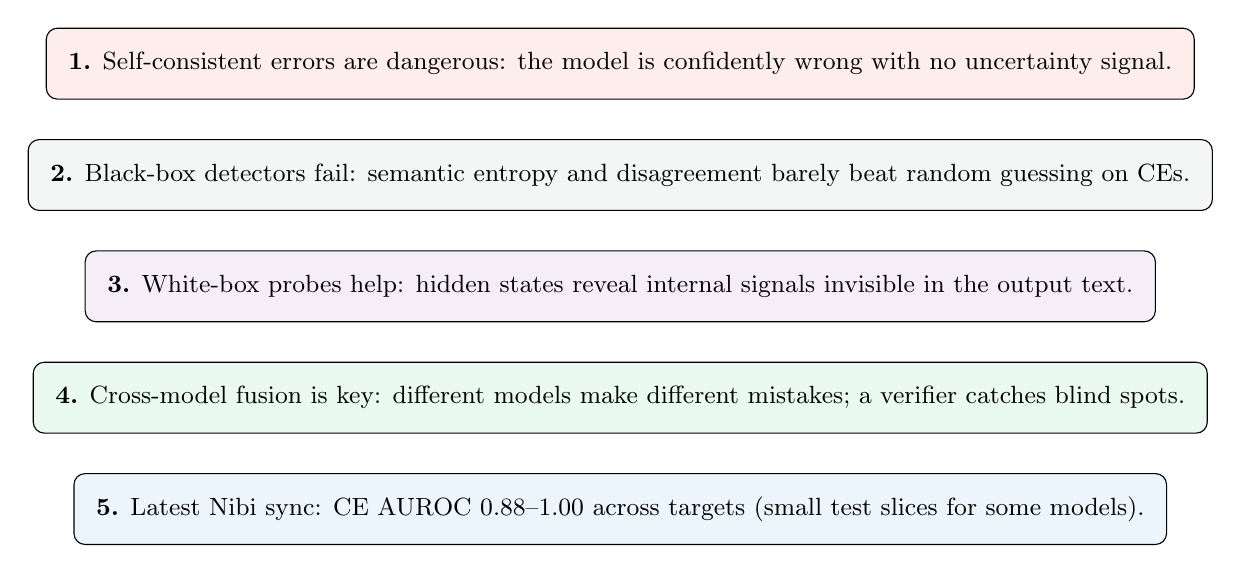
\begin{tikzpicture}[
    node distance=0.5cm,
    box/.style={rectangle, draw, rounded corners=4pt, minimum width=12cm, minimum height=0.9cm, align=left, font=\small, inner xsep=8pt},
]
    \node[box, fill=ceRed!10] (s1) {\textbf{1.} Self-consistent errors are dangerous: the model is confidently wrong with no uncertainty signal.};
    \node[box, fill=naGray!10, below=of s1] (s2) {\textbf{2.} Black-box detectors fail: semantic entropy and disagreement barely beat random guessing on CEs.};
    \node[box, fill=wbPurple!10, below=of s2] (s3) {\textbf{3.} White-box probes help: hidden states reveal internal signals invisible in the output text.};
    \node[box, fill=phase2Green!10, below=of s3] (s4) {\textbf{4.} Cross-model fusion is key: different models make different mistakes; a verifier catches blind spots.};
    \node[box, fill=phase1Blue!10, below=of s4] (s5) {\textbf{5.} Latest Nibi sync: CE AUROC 0.88--1.00 across targets (small test slices for some models).};
\end{tikzpicture}
\caption{Key takeaways from this work.}
\label{fig:summary}
\end{figure}

Tan et al.\ identified self-consistent errors as a critical blind spot for existing hallucination detectors and proposed cross-model probing as a solution. I adapted their method into my evaluation pipeline on TruthfulQA, maintaining consistency with my black-box measurements across six LLMs. In the latest synced Nibi batch (March 14, 2026), I have six completed all-target runs with fixed proxies (SmolLM3-3B + Phi-4-mini) and one Claude rerun with Qwen3.5-4B + Phi-4-mini. On the six-target CE batch, best-per-target CE AUROC averages 0.932, with some perfect scores on very small test subsets. These results continue to support the central claim: hidden-state probing, especially when combined with a verifier and fusion, can detect error patterns that black-box consistency signals miss.

\end{document}
